\textbf{\textit{Soal. }}Diberikan segitiga tumpul $ABC$ dengan $AB = BC$. Titik $D$ berada di dalam segitiga tersebut sedemikian sehingga $AD = BD$, $\angle ADB = 140^\circ$, dan $\angle ADC = 150^\circ$. Besar sudut $ACD$ dalam satuan $^\circ$ (derajat) adalah . . .
\begin{proof}[\textbf{Solusi 1. }] (Senin, 13 November 2023) Misalkan titik $E$ berada di dalam $\triangle BDC$ sedemikian sehingga $\triangle ABD \cong \triangle CBE$. 
% \begin{center}
    \begin{asy}
        import olympiad;
        import geometry;
        size(200);
        pair A, B, C, D, E;
        B = (0,8);
        A = (-9.534, 0);
        C = (9.534, 0);
        D = (-3.3111, 2.2649);
        E = (3.3111, 2.2649);
        draw(A--B--C--cycle);
        draw(E--B--D--cycle);
        draw(E--A--D--E--C--D);
        
        label("$A$", A, SW);
        label("$B$", B, N);
        label("$C$", C, SE);
        label("$D$", D, NW);
        label("$E$", E, NE);
    \end{asy}
\end{center}
\begin{center}
    \begin{tikzpicture}[scale=0.45, dot/.style={circle, fill, inner sep=0.5pt, outer sep=0pt}]

        \tkzDefPoint(0,8){B}
        \tkzDefPoint(-9.534,0){A}
        \tkzDefPoint(9.534,0){C}
        \tkzDefPoint(-3.3111,2.2649){D}
        \tkzDefPoint(3.3111,2.2649){E}

        \tkzDrawPolygon(A,B,C)
        \tkzDrawPolygon(E,B,D)
        \tkzDrawSegments(E,A A,D D,E E,C C,D)

        \tkzDrawPoints(A,B,C,D,E)
        \tkzLabelPoint[below left](A){$A$}
        \tkzLabelPoint[above](B){$B$}
        \tkzLabelPoint[below right](C){$C$}
        \tkzLabelPoint[above left](D){$D$}
        \tkzLabelPoint[above right](E){$E$}

    \end{tikzpicture}
\end{center}

Ini berarti $AD=EC$ dan $\angle DAC = \angle BAC - \angle BAD = \angle BCA - \angle BCE = \angle ECA$ sehingga $ADEC$ trapesium sama kaki yang jelas siklis. Lalu, $\angle BAD = \angle DBA = 20^\circ$. 

Sekarang misalkan $\angle DBE = 2x$ maka karena $AB=BC$ didapat $\angle DAC = \angle ECA = 50^\circ - x$. Lalu, karena $BD=BE$ maka $\angle BDE = \angle BED = 90^\circ-x$. Selanjutnya, $\angle EDC = 360^\circ - \angle ADC - \angle ADB - \angle BDE = x-20^\circ$. Oleh karena $ADEC$ siklis dan sama kaki, maka $\angle DEA = \angle EDC = x-20^\circ$.

Dari fakta tersebut didapat $\angle BEA = \angle BED + \angle DEA = 70^\circ = \frac{1}{2}\angle BDA$. Namun, karena $DB=DA$ maka didapat $D$ adalah pusat lingkaran $(ABE)$ sehingga $EB=BD=DE$ yang menyebabkana $\triangle BDE$ sama sisi sehingga $2x = \angle DBE = 60^\circ \implies x = 30^\circ$. 

Oleh karena itu karena $DECA$ siklis didapat $\angle ACD = \angle AED = x-20^\circ = 10^\circ$.
\end{proof}

\begin{proof}[\textbf{Solusi 2. }] (Senin, 13 November 2023) Perhatikan bahwa $\angle BDC = 360^\circ - \angle BDA - \angle ADC = 70^\circ$. Misalkan $\angle BCD = x$.
Dengan dalil sinus pada $\triangle BDC$ dan $\triangle ADB$ akan didapat
\begin{align*}
    \dfrac{\sin 140^\circ}{\sin 20^\circ} = \dfrac{\sin \angle ADB}{\sin \angle DAB} = \dfrac{AB}{BD} = \dfrac{BC}{BD} = \dfrac{\sin \angle BDC}{\sin \angle BCD} = \dfrac{\sin 70^\circ}{\sin x}
\end{align*}
sehingga didapat
\begin{align*}
    2\cos 20^\circ = \dfrac{2\sin 20^\circ \cos 20^\circ}{\sin 20^\circ} = \dfrac{\sin 40^\circ}{\sin 20^\circ} = \dfrac{\sin 140^\circ}{\sin 20^\circ} = \dfrac{\sin 70^\circ}{\sin x} = \dfrac{\cos 20^\circ}{\sin x}
\end{align*}
yang setara dengan
\begin{align*}
    \sin x = \frac{1}{2} \implies \angle DCB = x = 30^\circ \implies \angle DBC = 180^\circ - \angle BDC - \angle DCB = 80^\circ\\ \implies \angle ABC = \angle ABD + \angle DBC = 100^\circ \implies \angle BCA = \frac{1}{2}(180^\circ-\angle ABC) = 40^\circ\\ \implies \angle ACD = \angle BCA - \angle DCB = 10^\circ.
\end{align*}
% \begin{center}
    \begin{asy}
        import olympiad;
        import geometry;
        size(200);
        pair A, B, C, D, E, F;
        B = (0,8);
        A = (-9.534, 0);
        C = (9.534, 0);
        D = (-3.3111, 2.2649);
        draw(A--B--C--cycle);
        draw(A--D--B);
        draw(D--C);
        label("$A$", A, SW);
        label("$B$", B, N);
        label("$C$", C, SE);
        label("$D$", D, NW);

        markscalefactor=0.3;
        draw(anglemark(C,D,B), red);
        label("$70^\circ$", D+(1.5,0.7), red);

        markscalefactor=0.3;
        draw(anglemark(B,C,D), blue);
        label("$x$", C+(-2,0.8), blue);

        markscalefactor=0.1;
        label("$140^\circ$", D+(-0.5,0.2), blue);

        markscalefactor=0.15;
        label("$150^\circ$", D+(0.1, -1), orange);

        markscalefactor=0.3;
        draw(anglemark(D,A,B), blue);
        label("$20^\circ$", A+(1.5, 1), blue);
    \end{asy}
\end{center}
\begin{center}
    \begin{tikzpicture}[scale=0.45, dot/.style={circle, fill, inner sep=0.5pt, outer sep=0pt}]

        \tkzDefPoint(0,8){B}
        \tkzDefPoint(-9.534,0){A}
        \tkzDefPoint(9.534,0){C}
        \tkzDefPoint(-3.3111,2.2649){D}

        \tkzDrawPolygon(A,B,C)
        \tkzDrawSegments(A,D D,B D,C)

        % Tanda sudut
        \tkzMarkAngle[red,size=1.2](C,D,B)
        \tkzMarkAngle[blue,size=1.2](B,C,D)
        \tkzMarkAngle[blue,size=1.2](D,A,B)

        % Label sudut
        \tkzDefPoint(-1.8111,2.9649){l70}\tkzLabelPoint(l70){\textcolor{red}{$70^\circ$}}
        \tkzDefPoint(7.534,0.8){lx}\tkzLabelPoint(lx){\textcolor{blue}{$x$}}
        \tkzDefPoint(-3.8111,2.4649){l140}\tkzLabelPoint(l140){\textcolor{blue}{$140^\circ$}}
        \tkzDefPoint(-3.2111,1.2649){l150}\tkzLabelPoint(l150){\textcolor{orange}{$150^\circ$}}
        \tkzDefPoint(-8.034,1.0){l20}\tkzLabelPoint(l20){\textcolor{blue}{$20^\circ$}}

        \tkzDrawPoints(A,B,C,D)
        \tkzLabelPoint[below left](A){$A$}
        \tkzLabelPoint[above](B){$B$}
        \tkzLabelPoint[below right](C){$C$}
        \tkzLabelPoint[above left](D){$D$}

    \end{tikzpicture}
\end{center}


\end{proof}